\documentclass[12pt,a4paper]{article}

% ---------- Packages ----------
\usepackage[UTF8]{ctex} % Supports Chinese natively with XeLaTeX
\usepackage{geometry}
\usepackage{setspace}
\usepackage{hyperref}

% ---------- Page Setup ----------
\geometry{margin=1in}
\setstretch{1.25}

% ---------- Title ----------
\title{
    \Huge \textbf{Proof Documents Collection} \\[0.5cm]
    \Large Southern University of Science and Technology (SUSTech)
}

\author{By Lucky Chen}

\date{\today}

% ---------- Document ----------
\begin{document}

\maketitle
\thispagestyle{empty}

% ---------- Instructions ----------
\vspace{1cm}

\noindent \textbf{Instructions / 使用须知:}

\begin{itemize}
    \item Find each office’s email or contact the corresponding secretary. 请先查找各中心的官方邮箱或对应秘书联系方式。
    \item Alternatively, print this document and bring it to the office for detailed instructions and the official stamp (\textbf{盖章}).
    \item Note: Some centers (e.g., Sports Center) may prefer bilingual formatting: one line in Chinese, one line in English.
    \item For full Chinese support, please compile with \textbf{XeLaTeX}. 如需中文支持,请使用 XeLaTeX 编译;或直接使用提供的 Word 模板。
    \item You are encouraged to register for \textbf{语言指导服务} at the SUSTech Center for Language Education (CLE); they are very helpful with all kinds of application materials!
\end{itemize}

\vspace{1cm}

\noindent \textbf{Contact:} Lucky Chen \\
\texttt{yunwang.chen@email.com} 

\newpage

% ---------- Content ----------
\section{Scholarship Proof}
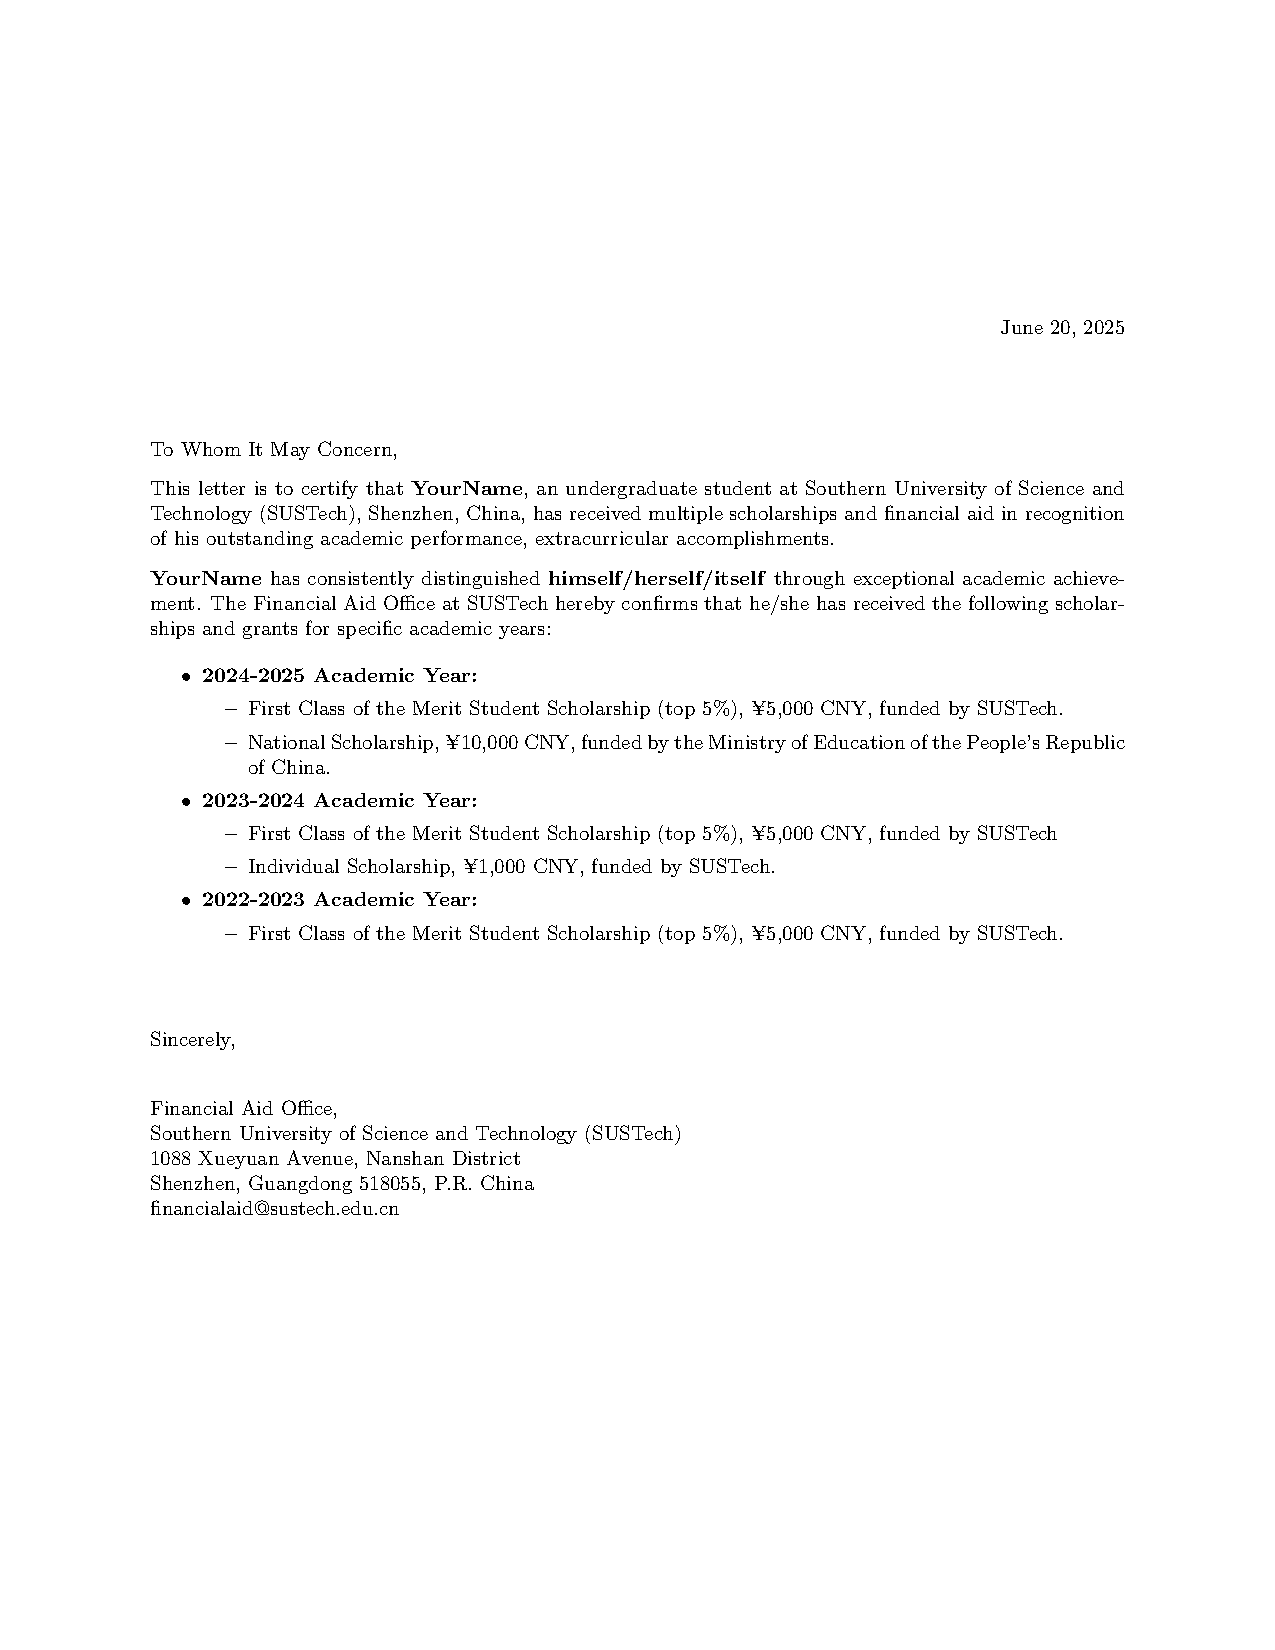
\includepdf[pages=-]{ScholarshipProof_FinancialAidOffice.pdf}

\section{Sports Awards Proof}
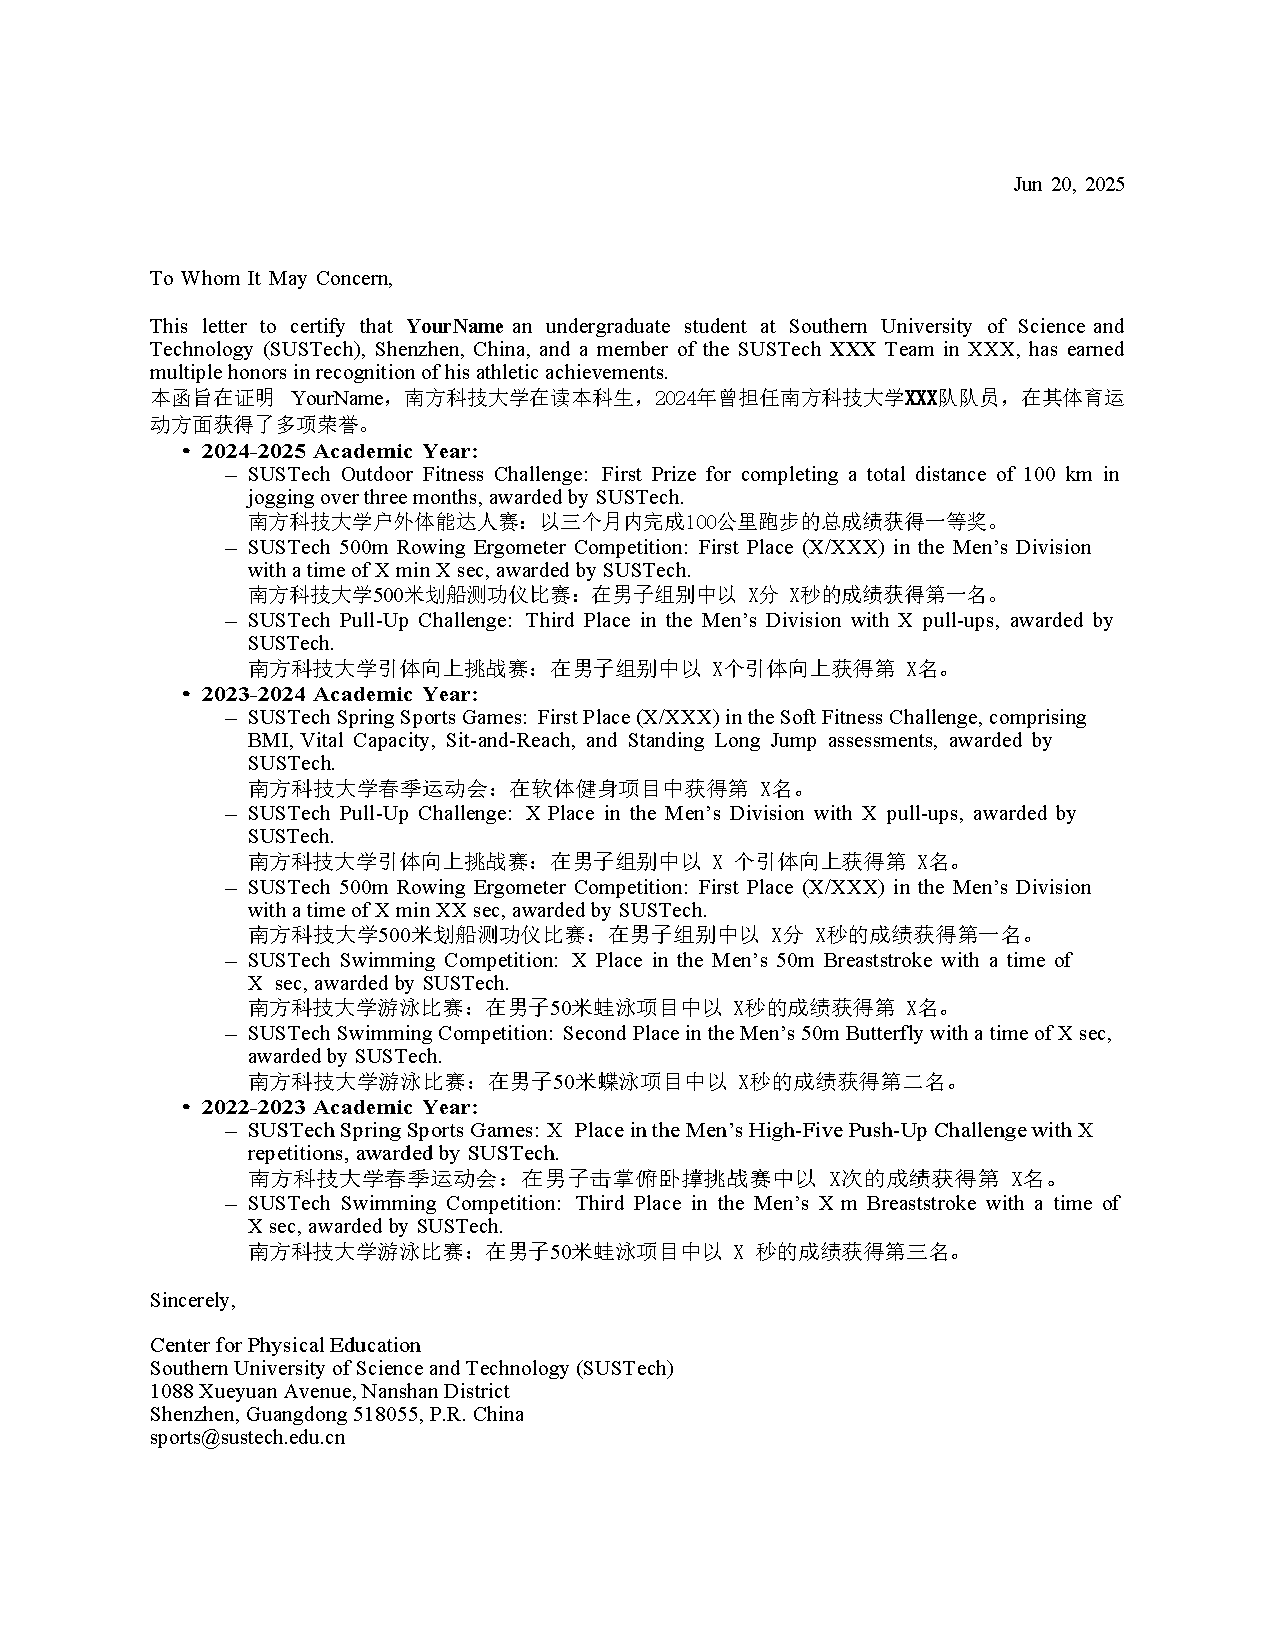
\includepdf[pages=-]{SportsAwardsProof_SportsCenter.pdf}

\section{SUSTech Admission Scholarship Proof}
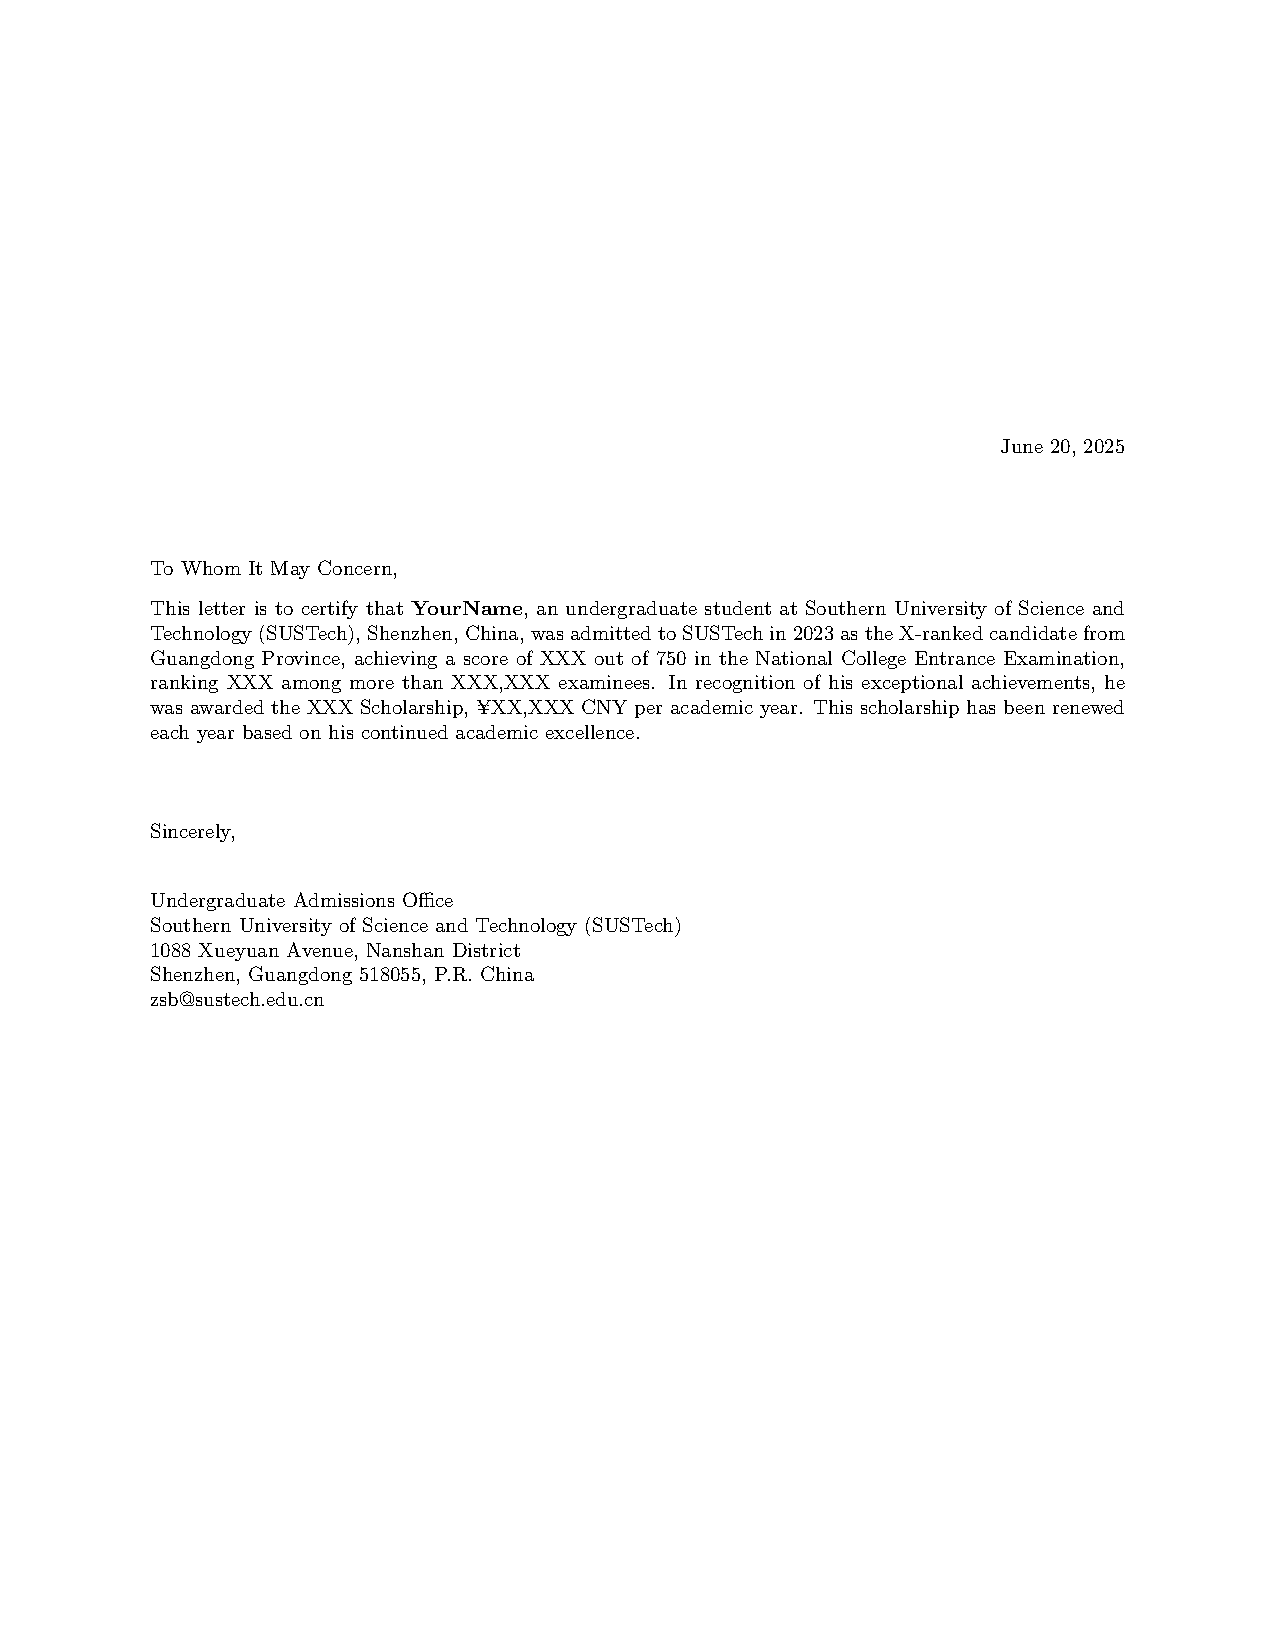
\includepdf[pages=-]{SUSTechAdmissionScholarshipProof_AdmissionOffice.pdf}

\section{SUSTech Volunteer Service Proof}
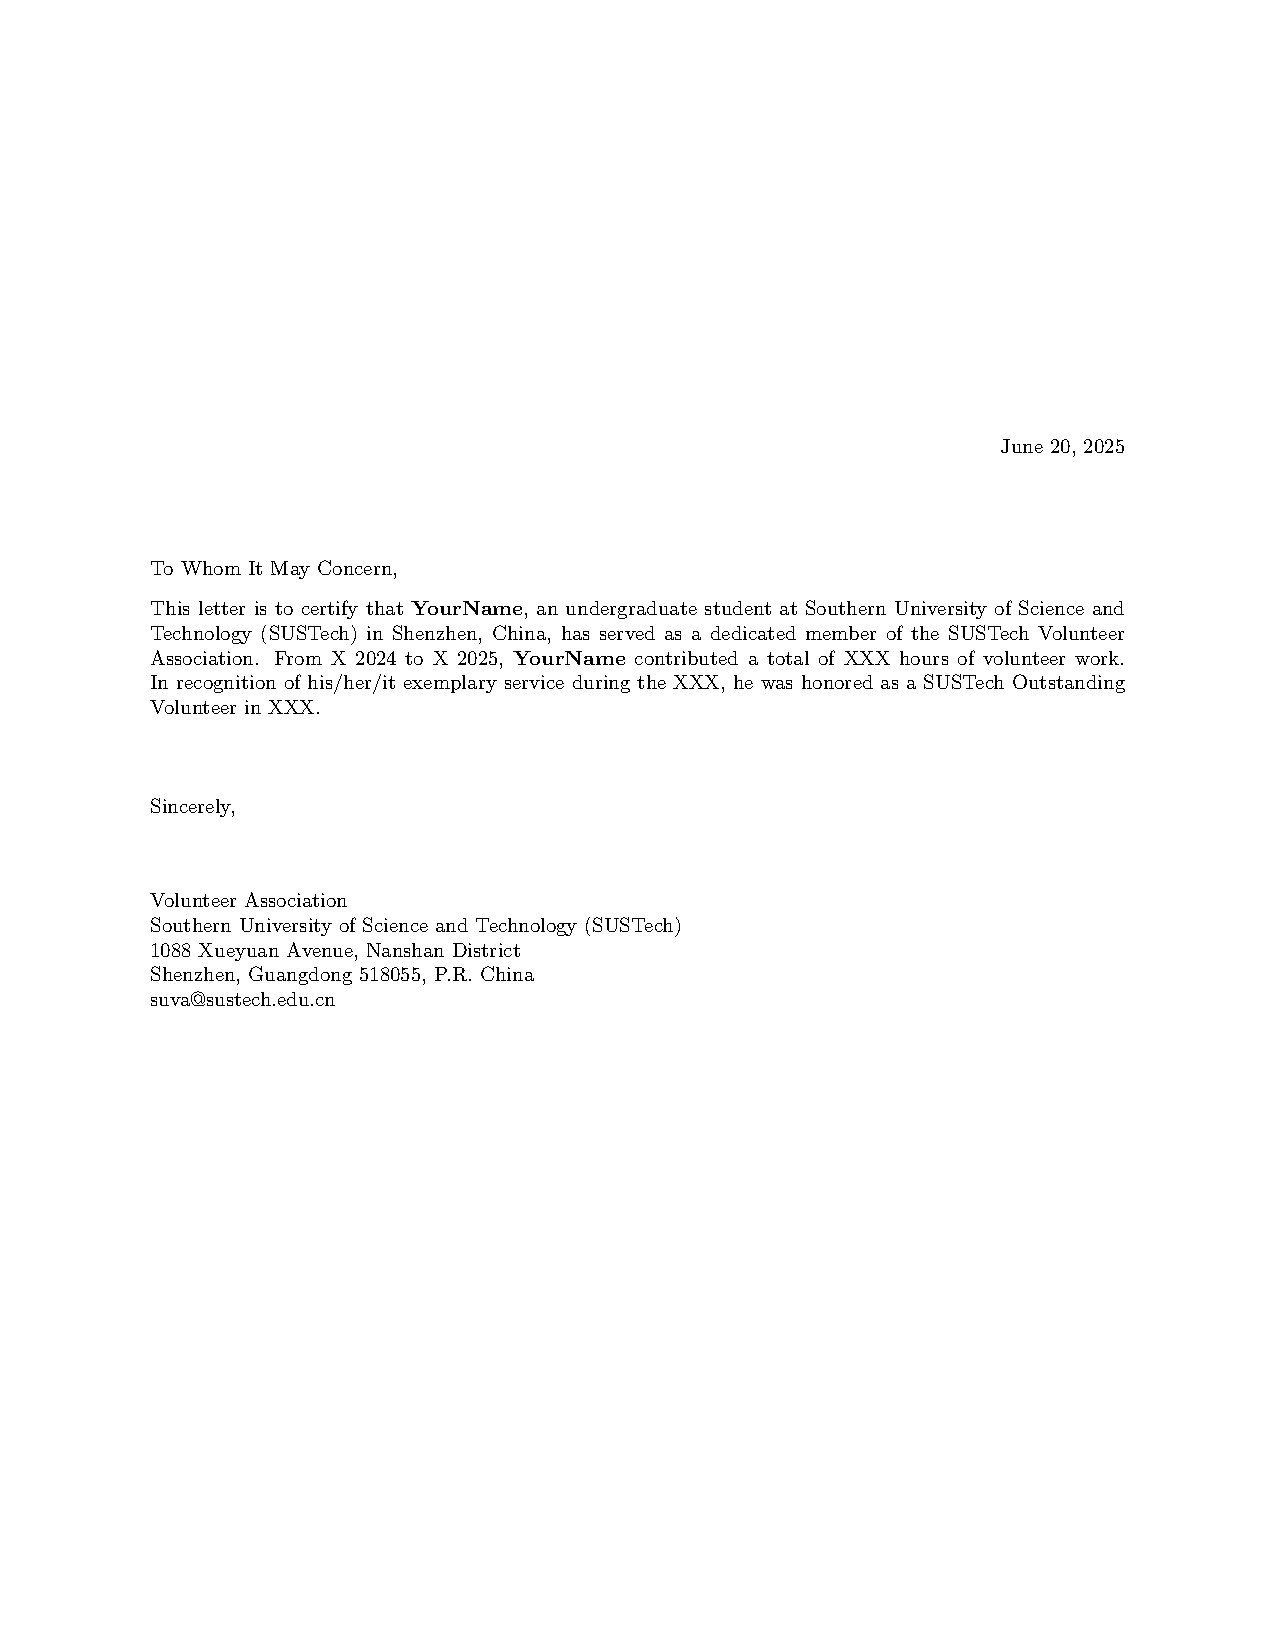
\includepdf[pages=-]{SUSTechVolunteerProof-SUSTechVolunteerAssociation.pdf}

% ---------- End ----------
\end{document}